

\begin{figure*}[t]
    \centering
    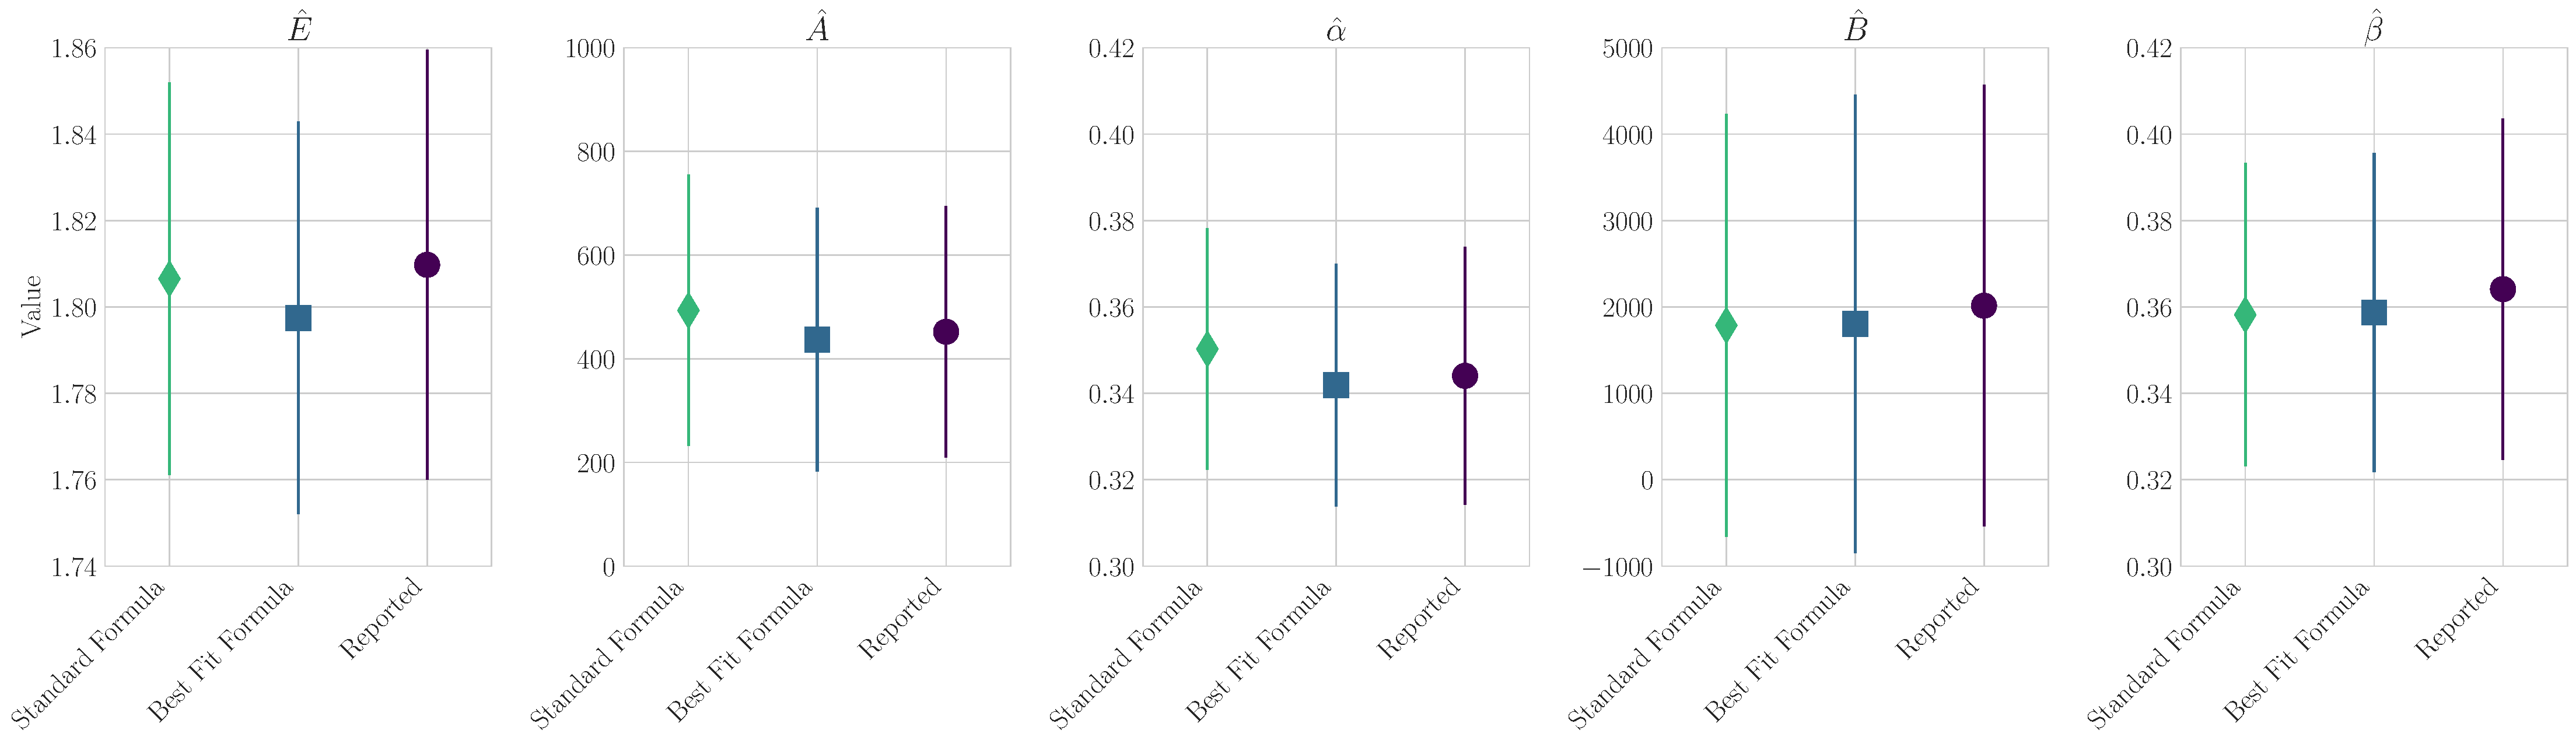
\includegraphics[width=0.85\linewidth]{figures/fit_parameters.pdf}
    \vspace{0.2cm}
    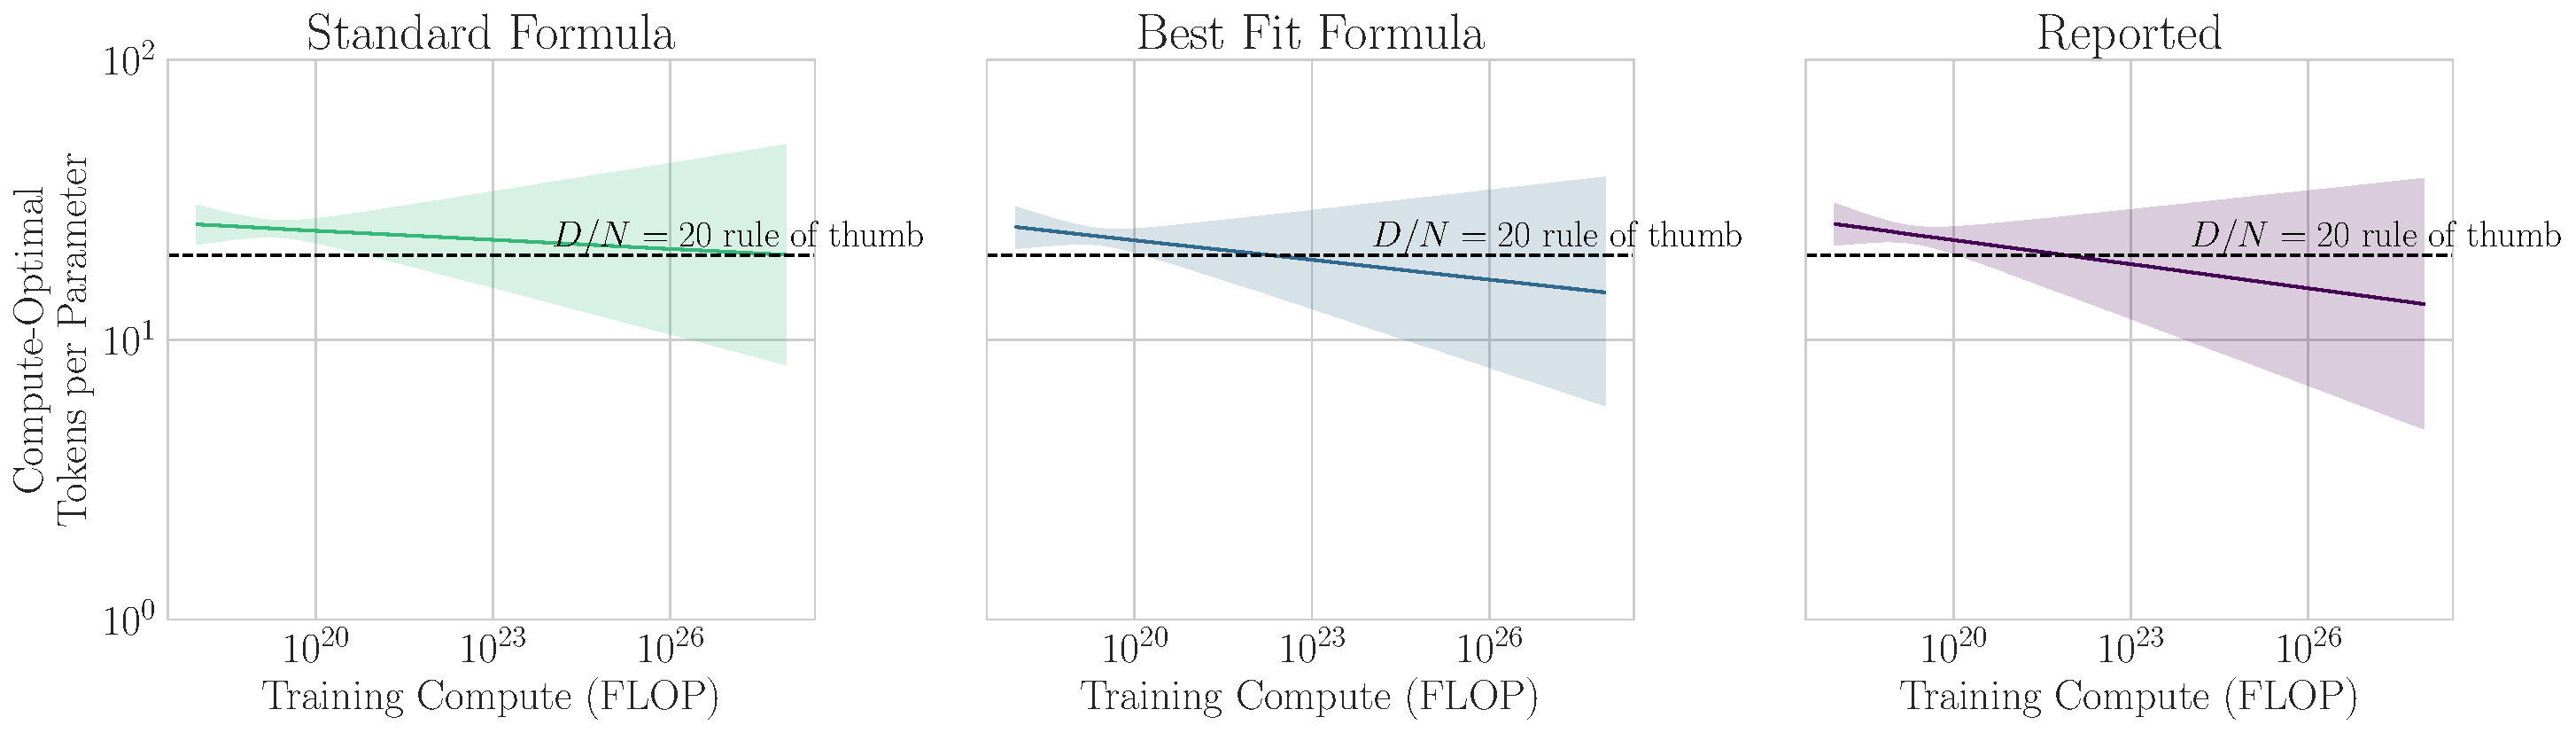
\includegraphics[width=\linewidth]{figures/compute_optimal_tokens_per_parameter_by_compute.pdf}
    \caption{\textbf{Key Chinchilla Results Are Robust to All Three Interpretations of Model Parameters.} \citet{hoffman2022chinchilla} fit a neural scaling law $L(N, D) = E + A \cdot N^{-\alpha} + B \cdot D^{-\beta}$, where $N$ is the number of model parameters and $D$ is the number of data (Eqn.~\ref{eqn:scaling_law}). \textbf{Top:} The fit parameters $(\hat{E}, \hat{A}, \hat{\alpha}, \hat{B}, \hat{\beta})$ do not meaningfully change, regardless of which model parameters are used for fitting. Error bars are standard errors from 4000 bootstrapped samples. \textbf{Bottom:} The compute-optimal tokens-per-parameter ratio remains constant at $\approx 20$, regardless of which notion of model parameters are used in the fitting process. 
    The slope is flattest with the standard formula model parameters ($-0.572$ per decade; best fit: $-1.049$; reported: $-1.248$).
    Error bars are 80\% confidence intervals. Fitting and visualization were conducted using \citet{besiroglu2024chinchillascalingreplicationattempt}'s \href{https://github.com/epoch-research/analyzing-chinchilla/}{code}.
    }
    \label{fig:results_dont_change}
\end{figure*}

\section{Key Chinchilla Results Are Robust to Three Interpretations of Chinchilla Model Parameters}
\label{sec:model_params_bestfit}

One of the fundamental inputs to the Chinchilla analyses are the number of parameters per model.
However, an ambiguity exists as to which exact model parameters were used, with three different possible interpretations differing by as much as 15.2\%.
We uncovered this by closely examining Chinchilla's Table A9, which reports the number of model parameters for each model alongside key architectural hyperparameters, e.g.,  d\_model, ffw\_size, kv\_size, n\_heads and n\_layers.
We call the model parameters reported in Chinchilla's Table A9 the \textbf{reported model parameters}.
We include a brief snippet in our main text (Table~\ref{tab:all_models_abridged}) and the full table in our Appendix~\ref{app:sec:chinchilla_table_a9}.

However, a second interpretation of the model parameters arises from the provided architecture hyperparameters. 
Assuming the embedding and unembedding weights are tied \citep{press2017using} and no gating is present, we can define a standard formula for the number of model parameters, denoted $N_{\text{std}}$, as the sum of embedding ($P_{\text{emb}}$), attention ($P_{\text{attn}}$), and feed-forward ($P_{\text{ffn}}$) parameters:
\begin{align}\label{eqn:standard}
    N_{\text{std}} &\approx P_{\text{emb}} + P_{\text{attn}} + P_{\text{ffn}} \\
    P_{\text{emb}} &= N_{\text{vocab}} \cdot d_{\text{model}} \nonumber \\
    P_{\text{attn}} &= n_{\text{layers}} \cdot (4 \cdot d_{\text{model}} \cdot d_{\text{kv}} \cdot n_{\text{heads}}) \nonumber \\
    P_{\text{ffn}} &= n_{\text{layers}} \cdot (2 \cdot d_{\text{model}} \cdot d_{\text{ff}}) \nonumber
\end{align}
\noindent where $V$ is the vocabulary size, $d_{\text{model}}$ is the model dimension, $d_{\text{kv}}$ is the key/value size, $n_{\text{heads}}$ is the number of heads, $n_{\text{layers}}$ is the depth, and $d_{\text{ff}}$ is the feed-forward width.

Comparing the \textbf{standard formula model parameters} ($N_{\text{std}}$) with the reported model parameters (denoted $N_{\text{reported}}$) reveals a mismatch for \textit{every} model, with an average relative error of 7.4\% but reaching as high as 15.2\% and no less than 3.6\% (Fig.~\ref{fig:model_params_bestfit}, left).
We calculate relative error as:
%
\begin{equation}
    \text{Relative Error (\%)} = 100 \cdot \frac{N_{\text{reported}} - N_{\text{std}}}{N_{\text{reported}}}
\end{equation}
%
In an attempt to reconcile the two interpretations of model parameters, we determined a third interpretation (denoted $N_{\text{best}}$) based on a ``best fit'' formula that nearly matches the reported model parameters. 
This formula is identical to Eq.~\ref{eqn:standard} except for the attention parameter count:
%
\begin{align}\label{eqn:bestfit}
    N_{\text{best}} &\approx P_{\text{emb}} + P_{\text{attn}} + P_{\text{ffn}} \\
    P_{\text{attn}} &= n_{\text{layers}} \cdot (\textcolor{red}{\mathbf{5}} \cdot d_{\text{model}} \cdot d_{\text{kv}} \cdot n_{\text{heads}}) \nonumber
\end{align}

Switching from the standard formula ($N_{\text{std}}$) to the \textbf{best fit model parameters} ($N_{\text{best}}$) reduced the number of discrepancies with the reported model parameters from $50/50$ models to $6/50$ models, and reduced the largest relative error from 15.2\% to 8.7\% (Fig.~\ref{fig:model_params_bestfit}, right).

We next tested how Chinchilla's results change depending on which of these three notions of model parameters are used for fitting.
We focus on two key results in particular:
First, Chinchilla fit a neural scaling law to the pretraining loss $L$ as a function of model parameters $N$ and pretraining data $D$:
%
\begin{equation}\label{eqn:scaling_law}
    L(N, D) = E + \frac{A}{N^{\alpha}} + \frac{B}{D^{\beta}},
\end{equation}
%
where $E$ is the irreducible error, $A$ is the parameter prefactor, $\alpha$ is the parameter exponent, $B$ is the data prefactor and $\beta$ is the data exponent. Second, Chinchilla derived from the estimated scaling law parameters a ``20-to-1'' heuristic for the compute-optimal ratio of tokens-per-parameters:
%
\begin{equation}
    D^* / N^* \approx 20
\end{equation}
%
We fit on the 50 Chinchilla configurations from Table A9 (reproduced in Appendix B) using publicly available \citet{besiroglu2024chinchillascalingreplicationattempt}'s \href{https://github.com/epoch-research/analyzing-chinchilla/}{Chinchilla fitting code and data} to test how these two Chinchilla headline results change depending on which of the three interpretations is used in the fits: (1)  Reported Model Parameters, (2) Standard Formula Model Parameters, or (3) Best Fit Formula Model Parameters.

Perhaps surprisingly, we found that none of the five fit parameters $\hat{E}, \hat{A}, \hat{\alpha}, \hat{B}, \hat{\beta}$ differed significantly depending on which of our three notions of model parameters were used in fitting (Fig.~\ref{fig:results_dont_change}, top).
We similarly found the compute-optimal tokens-per-parameter ratio remains constant around $20$ tokens per parameter (Fig.~\ref{fig:results_dont_change}, bottom).
Arguably, the standard formula model parameters yield a \textit{flatter} trend with increasing training compute: the slope for the standard formula model parameters is $-0.572$ for each 10x increase in compute, which decreased to $-1.049$ for the best fit formula model parameters and decreased further to $-1.248$ for the reported model parameters.
However, uncertainty makes drawing strong conclusions difficult.
These results demonstrate that \textbf{key Chinchilla results are robust to whichever of our three notions of model parameters is used in the fitting process}.